\documentclass[10pt,a4paper]{article}

\usepackage{polski}
\usepackage[utf8]{inputenc}
\usepackage[polish]{babel}
\usepackage{hhline}
\usepackage{pgfplots}
\usepackage{multicol}
\usepackage{graphicx}
\usepackage{caption}
\usepackage{subcaption}
\usepackage{colortbl}
\usepackage{geometry}
\usepackage{listings}
\usepackage{mathtools}
\DeclarePairedDelimiter\ceil{\lceil}{\rceil}
\DeclarePairedDelimiter\floor{\lfloor}{\rfloor}
\geometry{a4paper, total={170mm,257mm}, left=20mm, top=20mm }


\author{Sebastian Maciejewski 132275 i Jan Techner 132332\\
grupa I1, zajęcia w środy o 9:45}
\title{Przetwarzanie rozproszone - projekt “Obsługa Pyrkonu”}
\date{15 maja 2019}
\setlength{\parindent}{0pt}
\newcommand{\forceindent}{\leavevmode{\parindent=3em\indent}}
\begin{document}
\maketitle
\section{Opis problemu}
Zadanie polega na implementacji systemu zarządzania biletami na Pyrkon i warsztaty, które się na nim odbywają. 
Procesy (uczestnicy) ubiegają się o jeden z b biletów na Pyrkon, a następnie na kilka z rozróżnialnych warsztatów, 
z których każdy ma ograniczoną liczbę miejsc. Liczba warsztatów, miejsc na warsztatach i biletów na Pyrkon jest
przed każdym Pyrkonem losowana przez proces, który uruchamia wątek losowania biletów.
Poniżej przedstawiony jest opis algorytmu i schemat, który dokładnie obrazuje działanie programu.\\
\\
Działanie algorytmu rozpoczyna się od zgłoszenia przez każdy z procesów chęci rozpoczęcia nowego Pyrkonu.
W tym celu każdy proces wysyła wiadomość typu WANT\_TO\_BE\_HOST zawierającą znacznik czasowy wysłania wiadomości 
i czeka na $p-1$ ($p$ jest ilością procesów) wiadomości od innych procesów. Po otrzymaniu wszystkich wiadomości 
kązdy proces sprawdza czy jego znacznik czasowy jest największy i jeżeli tak, to proces zostaje hostem Pyrkonu.\\
\\
Następnym krokiem jest inkrementacja numeru Pyrkonu - jest on wykorzystywany do odrzucania przestarzałych wiadomości, które mogłyby zaburzyć działanie programu.
W naszej implementacji host wysyła wiadomość PYRKON\_START do pozostałych procesów,
po której odebraniu procesy inkrementują swoje numery Pyrkonu. Następnie host zwiększa swój numer Pyrkonu i tworzy wątek losujący.\\
\\
Ta procedura jest zobrazowana w górnej części poniższego diagramu, dodatkowy wątek (zaznaczony na niebiesko)
losuje ilość warsztatów, biletów na warsztaty i ilość biletów na Pyrkon, po czym przekazuje ją
wszystkim procesom za pomocą wiadomości PYRKON\_TICKETS i WORKSHOPS\_TICKETS. Wykorzystany w tym miejscu semafor (odblokowywany w momencie, gdy wszystkie procesy otrzymają
potwierdzenie otrzymania kompletnej informacji o biletach od innych procesów - GOT\_TICKETS\_INFO) służy wyrównaniu szans procesów na wejście na Pyrkon.\\
Dopiero wtedy mamy pewność, że wszyscy mają ten
sam numer Pyrkonu i te same (aktualne) informacje o biletach - można zatem rozpocząć procedurę 
ubiegania się o bilety.\\
\\
Każdy z Procesów informuje pozostałe o chęci wejścia na konwent (za pomocą wiadomości WANT\_PYRKON\_TICKET)
i po otrzymaniu odpowiedniej ilości ($p-b$) pozytywnych odpowiedzi zajmuje bilet. Następuje losowanie
ilości warsztatów, w których proces chce wziąć udział, po czym rozpoczyna się procedura ubiegania
się procesu o bilet na warsztaty. Jak widać na poniższym diagramie, kroki, które wykonuje proces są 
podobne do tych przy pobieraniu biletu na Pyrkon. Głównymi różnicami są tu typy wiadomości i fakt, że 
proces czeka na $p-w_i$ wiadomości ze zgodą na wejście na warsztat, gdzie $w_i$ to ilość biletów na $i$-ty warsztat.\\
Po otrzymaniu biletu i odczekaniu losowej ilości czasu (kiedy bierze udział w warsztacie), proces 
zwalnia bilet i, jeśli chce wziąć udział w jeszcze jakimś warsztacie, ponownie ubiega się o bilet,
tym razem na kolejny, losowo wybrany, warsztat. Jeżeli proces przeszedł już wszystkie warsztaty, którymi był
zainteresowany, wówczas zwalnia bilet na Pyrkon (wysyła odpowiedź ze zgodą na wejście oczekującym procesom)
i wraca do momentu, w którym ubiegał się o zostanie hostem. Kiedy wszystkie procesy opuszczą Pyrkon,
cały opisany proces rozpoczyna się od nowa.


\newpage
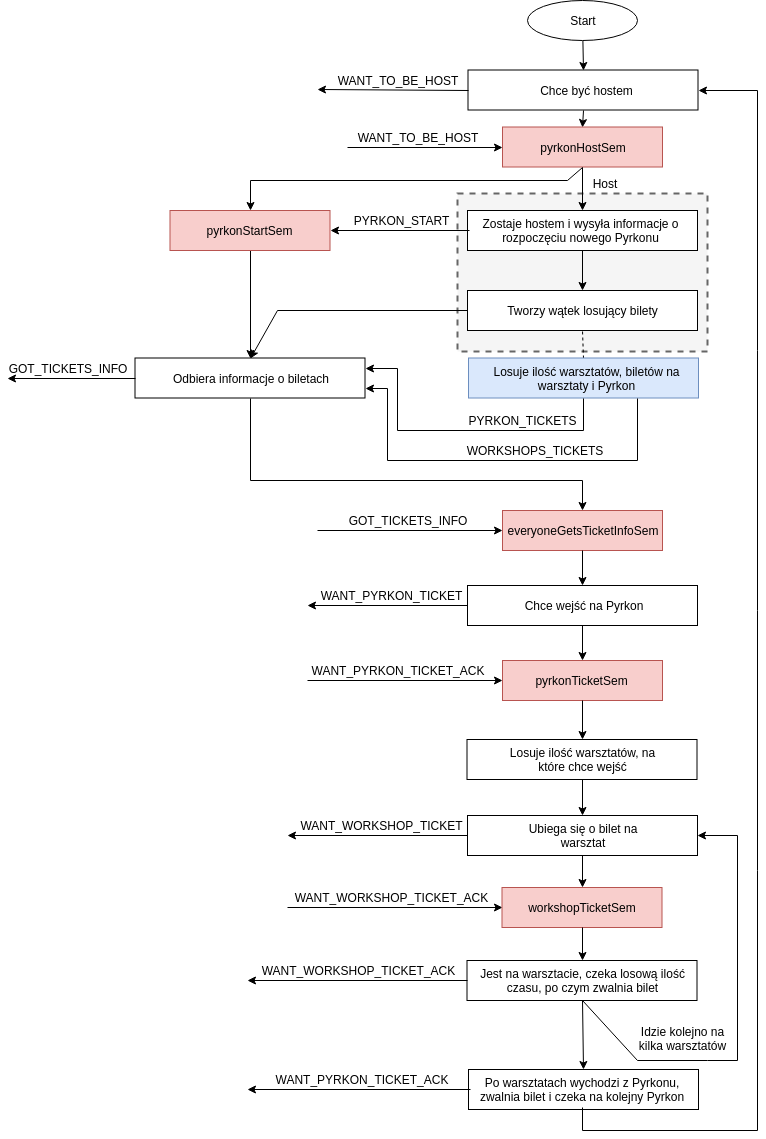
\includegraphics[height=\textheight]{diagram.png}
\newpage

\section{Założenia na temat środowiska}
W naszym rozwiązaniu zakładamy, że kolejki komunikatów są \textbf{FIFO} i kanały komunikacji są niezwaodne o nieskończonej pojemności.
Należy jednak zauważyć, że zastosowanie semaforów, na których proces musi czekać na wszystkie pozostałe procesy, w rzeczywistości ogranicza
maksymalną ilość wiadomości obecnych jednocześnie w systemie.

\section{Złożoność komunikacyjna i czasowa}
W pojedynczym Pyrkonie można wyznaczyć ilości wysyłanych komunikatów - przy założeniu, że $p$ to ilość procesów a $w$ to ilość warsztatów,
złożoność komunikacyjna jest dla pszczególych typów wiadomości następująca:\\
\begin{itemize}
    \item $p \cdot (p-1)$ - WANT\_TO\_BE\_HOST
    \item $(p-1)$ - PYRKON\_START
    \item $p + p + w\cdot p$ - informacje o biletach (ilość warsztatów, biletów na Pykon i ilość biletów na każdy warsztat)
    \item $p \cdot (p-1)$ - GOT\_TICKETS\_INFO
    \item $p \cdot [(p-1) + (p-1)]$ - WANT\_PYRKON\_TICKET i WANT\_PYRKON\_TICKET\_ACK
    \item $p \cdot (w-1) \cdot [(p-1) + (p-1)$] - WANT\_WORKSHOP\_TICKET i WANT\_WORKSHOP\_TICKET\_ACK
\end{itemize}
Sumaryczna (pesymistyczna) ilość komunikatów wysyłanych w ciągu jednego Pyrkonu to
$2p^2 (w+1) + p(1-w) - 1$\\

Podobnie można opisać złożoność czasową (w pesymistycznym przypadku - gdy na Pyrkon jest tylko jeden bilet i każdy proces idzie na $w-1$ warsztatów):\\
\begin{itemize}
    \item $1$ - WANT\_TO\_BE\_HOST
    \item $1$ - PYRKON\_START
    \item $1 + 1 + w$ - informacje o biletach (ilość warsztatów, biletów na Pykon i ilość biletów na każdy warsztat)
    \item $1$ - GOT\_TICKETS\_INFO
    \item $1 + p$ - WANT\_PYRKON\_TICKET i WANT\_PYRKON\_TICKET\_ACK
    \item $p\cdot (1+1) \cdot w$ - WANT\_WORKSHOP\_TICKET i WANT\_WORKSHOP\_TICKET\_ACK
\end{itemize}

Złożoność czasowa w pesymistycznym przypadku (na Pyrkon jest tylko jeden bilet) to $6 + w + p + 2 p w$

\end{document}